\documentclass{unicam_thesis}
\usepackage[utf8]{inputenc}
\usepackage{listings}
%\usepackage[backend=bibtex]{biblatex}
%%%%%%%%%%%%%%%%%%%%%%%%%%%%
% TESI DATI FRONTESPIZIO
%%%%%%%%%%%%%%%%%%%%%%%%%%%%

\title{INTEGRAZIONE MICROSOFT DIAL SU DASHBOARD LOCCIONI }

\university{Universit\`a degli Studi di Camerino}%
\school{Scienze e Tecnologie}%
\course{Laurea in Informatica (Classe L-31)}%

\author{Daniele Moschini}%
\advisor{Prof. Michele Loreti}%
\coadvisor2{Luca Mazzuferi}%
\academicyear{2020/2021}%
\matricola{101439}

%%%%%%%%%%%%%%%%%%%%%%%%%%%%
% FINE DATI FRONTESPIZIO
%%%%%%%%%%%%%%%%%%%%%%%%%%%%

\theoremstyle{definition} \newtheorem{esempio}{Esempio}[chapter]
\theoremstyle{definition}
\newtheorem{definizione}{Definizione}[chapter] \theoremstyle{plain}
\newtheorem{teorema}{Teorema}[chapter]

\graphicspath{{Screenshot/},{Immagini/},{API/},{Source/}}
\bibliography{biblio.bib}
%\addbibresource{biblio.bib}

\begin{document}

\maketitle

\tableofcontents
\lstlistoflistings
\listoffigures
\listoftables

\chapter{Introduzione}
\label{chap:intro}

Negli ultimi anni, lo sviluppo e controllo di software aziendali si sta spostando in maniera decisa verso il Web, permettendo una maggior portabilità e scalabilità in termini di sviluppo e riutilizzo, consentendo il controllo da remoto tramite qualsiasi dispositivo connesso alla rete. Di conseguenza l’utilizzo di dispositivi di input che si basano sul protocollo HID é sempre piú richiesto e talvolta necessario anche in ambienti Web, per una miglior esperienza utente e una maggior precisione nelle operazioni.
Durante il nostro periodo di Stage++ svolto presso l'impresa \emph{Loccioni} \cite{Loc}, ci é stato proposto di analizzare le possibili strade da percorre al fine di integrare un dispositivo Microsoft, in particolare il \emph{Surface Dial}\cite{dial}, all'interno delle loro Dashbord, utilizzate per la visualizzazione e la manipolazione dei dati durante le fasi di testing su componenti elettronici.
\begin{center}

\includegraphics[width=0.5\textwidth]{loccioni}
\end{center}

\newpage
\section{Obiettivo}
Attualmente nei banchi prova dove vengono effettuati i test su componenti elettrici di Automobili, lo strumento principale per la variazione dei dati é rappresentato da una pulsantiera, composta da potenziometri analogici, bottoni e switch, i quali rappresentano delle evidenti limitazioni in termini  di usabilità e sicurezza.Per questo motivo, attraverso una digitalizzazione della pulsantiera e l'utilizzo di un dispositivo di precisione, l'utilizzo finale di un banco prova risulterebbe piú sicuro e semplice da utilizzare per l'operatore, migliorandone l'efficienza e la precisione con conseguente risparmio in termini di tempo e denaro.\\

L'elaborato in questione ha quindi come obbiettivo l'integrazione del dispositivo Microsoft \textbf{Surface Dial} nei software Web Loccioni, in particolare nelle Dashboard utilizzate nei banchi prova per la visualizzazione e la manipolazione dei dati, con lo scopo di rendere piú fluida e intuitiva l'esperienza utente e consentendo all'operatore finale di svolgere operazioni in parallelo, attraverso l'utilizzo di entrambe le mani, mantenendo il focus di un dispositivo su un determinato compito.\\

A tal proposito, per rendere possibile tale integrazione é stato necessario svolgere un fase di analisi del dispositivo da integrare e della Dashboard sulla quale verrá utilizzato. Quello che ne risulta, é un servizio ideato e sviluppato con lo scopo principale di permettere la comunicazione tra il dispositivo HID in questione e una qualsiasi pagina Web.

\newpage
\section{Analisi e Studio di Fattibilità}

L'idea iniziale era quella di utilizzare il Dial per il controllo di macchinari, che attualmente fanno uso di programmi Windows Forms per la manipolazione dei dati, mentre si appoggiano ad un loro Framework Web per la visualizzazione in tempo reale dei dati stessi.\\

Per prima cosa ci siamo dedicati alla lettura della documentazione scritta da Microsoft \cite{dialdoc} e siamo giunti alla conclusione che le funzionalità base del Dial sono quattro eventi principali:

\begin{itemize}
\item \textbf{Click}: Pressione rapida del bottone presente nel dispositivo.
\item \textbf{Pressione prolungata}: Pressione prolungata del bottone presente nel dispositivo.
\item \textbf{Rotazione}: Evento rotazione che avviene ruotando il dispositivo
\item \textbf{Posizionamento sullo schermo}: Il dispositivo può essere appoggiato in alcuni schermi compatibili ed essere riconosciuto dal sistema.
\end{itemize}

Una volta individuate le potenzialità del Dial, abbiamo iniziato una fasi di testing su applicazioni native\cite{uwpex} per comprendere come e dove potevamo utilizzare le librerie messe a disposizione per il dispositivo, con la successiva creazione di un piccolo prototipo che sfruttasse e mostrasse le suddette funzionalità.\\

Successivamente ci siamo dedicati alla comunicazione tra un qualsiasi tipo di ambiente software e il Dial, scoprendo che il dispositivo comunica attraverso il protocollo HID con qualsiasi Hardware, ma senza l'utilizzo della Libreria RadialController, si vanno a perdere tutte quelle funzionalità che permettono l'utilizzo completo del Dial, rendendolo meno necessario in termini di miglioramento della User Experience.
 
\subsection{Ricerca}


Durante lo studio di fattibilità, ci siamo dedicati alla ricerca di progetti che utilizzassero il Dial \cite{son} indifferentemente dall’ambiente, da quello grafico a quello audio, trovando solamente un programma che permettesse l'utilizzo del Dial in un Sintetizzatore Software\cite{el}, attraverso il protocollo MIDI, limitando il controllo alla semplice rotazione e pressione, togliendo tutte quelle funzionalità più interessanti, come il posizionamento del dispositivo sullo schermo e la visualizzazione dinamica del Menu in relazione alla posizione in cui trova.\\

Per questo motivo, abbiamo deciso in concordato con i nostri tutor Aziendali di non gestire noi la comunicazione tra dispositivo e software, ma di lasciare questo compito alle librerie messe a disposizione da Microsoft.

Dato il crescente sviluppo dell'utilizzo di applicazioni web e del relativo controllo delle stesse attraverso dispositivi HID, abbiamo quindi proseguito con la ricerca per l'integrazione dei suddetti dispositivi nel mondo Web, accantonando per il momento, la possibilitá di integrarlo negli applicativi Windows Forms Loccioni, anche a causa del necessario refactoring di tutte le applicazioni che intendessero utilizzarlo.\\

Considerando che il posizionamento su schermo è supportato solamente da determinati dispositivi Microsoft ( Surface Studio, Surface Pro 4/5/6, ...) abbiamo pensato di creare un’applicazione UWP (Universal Windows Platform) che potesse girare nativamente su tali dispositivi. Per poter infine, acquisire il controllo di una pagina web, abbiamo deciso di utilizzare una WebView avviata a RunTime permettendo all'utente di poter utilizzare il Dial sui dispositivi che supportano l'interazione con lo schermo grazie alle Librerie Native, ma anche di poterla utilizzare senza l'utilizzo del Dial, attraverso un qualsiasi browser web.

\newpage
\section{Struttura della Tesi}
L'esposizione del seguente documento sará cosi suddivisa:
\begin{itemize}
\item Il capitolo \emph{Metodologie e strumenti di sviluppo}\autoref{chap:metod} espone la metodologia utilizzata per lo sviluppo del lavoro in team e descrive le tecnologie utilizzate nel corso del progetto.
\item Il capitolo \emph{Architettura}\autoref{chap:serv} descrive la struttura del progetto e in dettaglio le funzionalità implementate grazie ad esso.
\item Il capitolo \emph{Conclusione}\autoref{chap: Conclusioni} racchiude le considerazioni critiche sul lavoro svolto ed espone delle possibili implementazioni future atte a migliorare il servizio.
\end{itemize}








\chapter{Metodologie e Strumenti Di Sviluppo}
\label{chap:metod}

\section{Metodologie di Sviluppo}
Durante lo sviluppo del progetto abbiamo utilizzato uno sviluppo Scrum\cite{scr} unito al modello incrementale, utilizzando un Scrum per quanto riguarda la distribuzione del lavoro e il rapporto con l'azienda, mentre il rilascio incrementale è stato utilizzato una volta scoperte tutte le potenzialità del Dial e il corretto funzionamento su pagine web.

\subsection{Scrum}
 
Scrum è un framework agile per la gestione del ciclo di sviluppo del software, iterativo ed incrementale, concepito per gestire progetti e prodotti software o applicazioni di sviluppo, creato e sviluppato da Ken Schwaber e Jeff Sutherland.\\

\begin{figure}[htpb!]
\center
  
\includegraphics[width=0.4\textwidth]{Scrum}
  \caption{Scrum}
\end{figure}

Scrum enfatizza tutti gli aspetti di gestione di progetto legati a contesti in cui è difficile pianificare in anticipo. Vengono utilizzati meccanismi propri di un "processo di controllo empirico", in cui cicli di feedback che ne costituiscono le tecniche di management fondamentali risultano in opposizione alla gestione basata sul concetto tradizionale di command-and-control. Il suo approccio alla pianificazione e gestione di progetti è quello di portare l'autorità decisionale al livello di proprietà e certezze operative.\\

Sono 3 i ruoli che vengono individuati nella metodologia Scrum: \emph{Product Owner}, \emph{Scrum Master} e \emph{Team di Sviluppo}:

\begin{itemize}
\item Il \textbf{Product Owner} definisce il lavoro da svolgere e l'ordine con cui viene completato. Raccoglie la voce degli stakeholder (clienti, management e chiunque abbia un interesse nel prodotto), le necessità dell'utente finale, i requisiti del mercato e sulla base di questi elementi stabilisce le priorità di sviluppo per il Team Scrum.
\item Lo \textbf{Scrum Master} è il responsabile del processo, e un leader a servizio (servant-leader) dello Scrum Team. Conoscitore esperto della metodologia Scrum, sa come applicarla e si assicura che il Team comprenda e segua le regole che la caratterizzano, perché il progetto abbia successo. Inoltre favorisce il lavoro del Team di Sviluppo, rimuovendo ostacoli, organizzando meeting di confronto, e soprattutto proteggendolo da ogni possibile distrazione: ogni membro del gruppo deve poter lavorare al 100 per 100 sullo sviluppo, e lo Scrum Master si assicura che questo avvenga.
\item Il \textbf{Team di Sviluppo} è la squadra di lavoro, composta da 3 a 9 persone. Anche lo Scrum Master può far parte del Team di Sviluppo. Chi concretamente porta a termine gli Sprint e fornisce le funzionalità da implementare è questo insieme coordinato di persone, autogestito e cross-funzionale.
\end{itemize}

Per quanto riguarda il nostro progetto, abbiamo applicato il framework Scrum con i ruoli definiti nel seguente schema:
\begin{itemize}
\item \textbf{Product Owner}: Luca Mazzuferi
\item \textbf{Scrum Master}: Marco Allegrezza, Diego Bonura
\item \textbf{Team di Sviluppo}: Daniele Moschini, Michele Benedetti
\end{itemize}

\newpage
\subsection{Rilascio Incrementale}

Per \textbf{modello incrementale}\cite{rin} si intende, nell'ambito dell'ingegneria del software, un modello di sviluppo di un progetto software basato sulla successione dei seguenti passi principali:

\begin{itemize}
\item Pianificazione
\item Analisi dei requisiti
\item Progetto
\item Implementazione
\item Prove
\item Valutazione
\end{itemize}

Questo ciclo può essere ripetuto diverse volte, in cui ogni "incremento" riduce il rischio di fallimento e produce nuovo valore. Il ciclo viene ripetuto fino a che la valutazione del prodotto diviene soddisfacente rispetto ai requisiti previsti.\\

L'utilizzo del modello incrementale è consigliabile quando si ha, fin dall'inizio della progettazione, una visione abbastanza chiara dell'intero progetto, perché occorre fare in modo che la realizzazione della generica versione k risulti utile per la realizzazione della versione k+1.\\

Un approccio incrementale è particolarmente indicato in tutti quei casi in cui la specifica dei requisiti risulti particolarmente difficoltosa e di difficile stesura (semi)formale. L'uso di questo modello di sviluppo favorisce la creazione di prototipi, ovvero parti di applicazione funzionanti, che a loro volta favoriscono il dialogo con il cliente e la validazione dei requisiti.

\begin{figure}[htpb!]
\center
  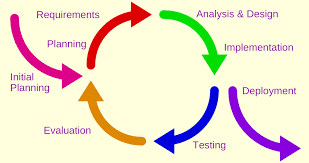
\includegraphics[width=0.6\textwidth]{RilascioIncrementale}
  \caption{Rilascio Incrementale}
\end{figure}

\newpage
\section{Strumenti utilizzati}

Durante lo sviluppo del progetto, sono state utilizzate varie tecnologie, strumenti, linguaggi e relativi framework che verranno dettagliatamente descritti di seguito.

\subsection{Microsoft Dial}

\begin{figure}[htpb!]
\center
  \includegraphics[width=0.4\textwidth]{Dial}
  \caption{Microsoft Dial}
\end{figure}

Il Microsoft Surface Dial\cite{dial} é un dispositivo di rotazione proprietario Microsoft, ideato per l'utilizzo con la mano secondaria durante le attivitá di progettazione e modifica dati. Composto da un sensore laser che permette di calcolare 3600 punti di precisione grazie alla sua riflessione e da un sistema di vibrazione haptico che restituisce un feedback tattile durante l'utilizzo. Nella parte inferiore presenta un plate in silicone ideato per generare la giusta aderenza durante il contatto con display inclinati.\\

\begin{figure}[htpb!]
	\begin{minipage}{0.35\textwidth}
		\centering
		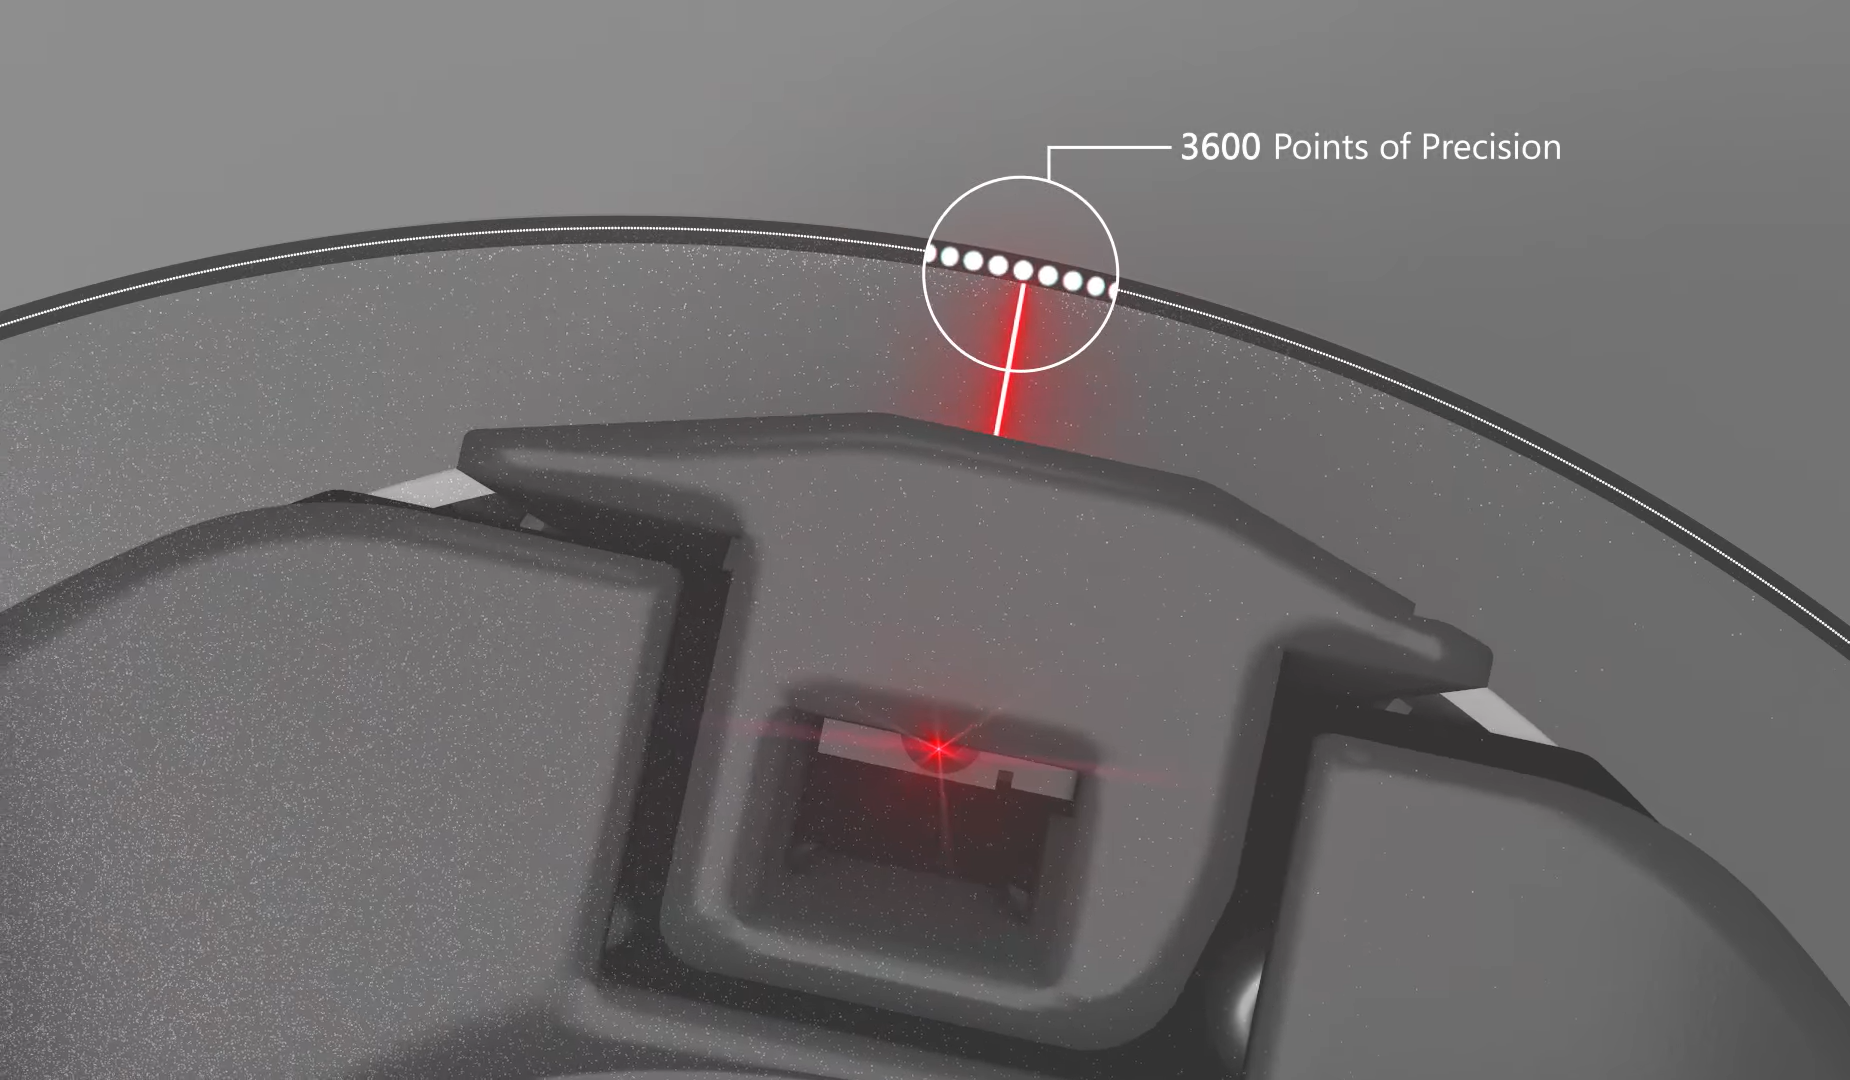
\includegraphics[width=0.9\textwidth]{DialPoint}
		\caption{Dial laser point}
    \end{minipage}\hfill
    \begin{minipage}{0.65\textwidth}
		\centering
		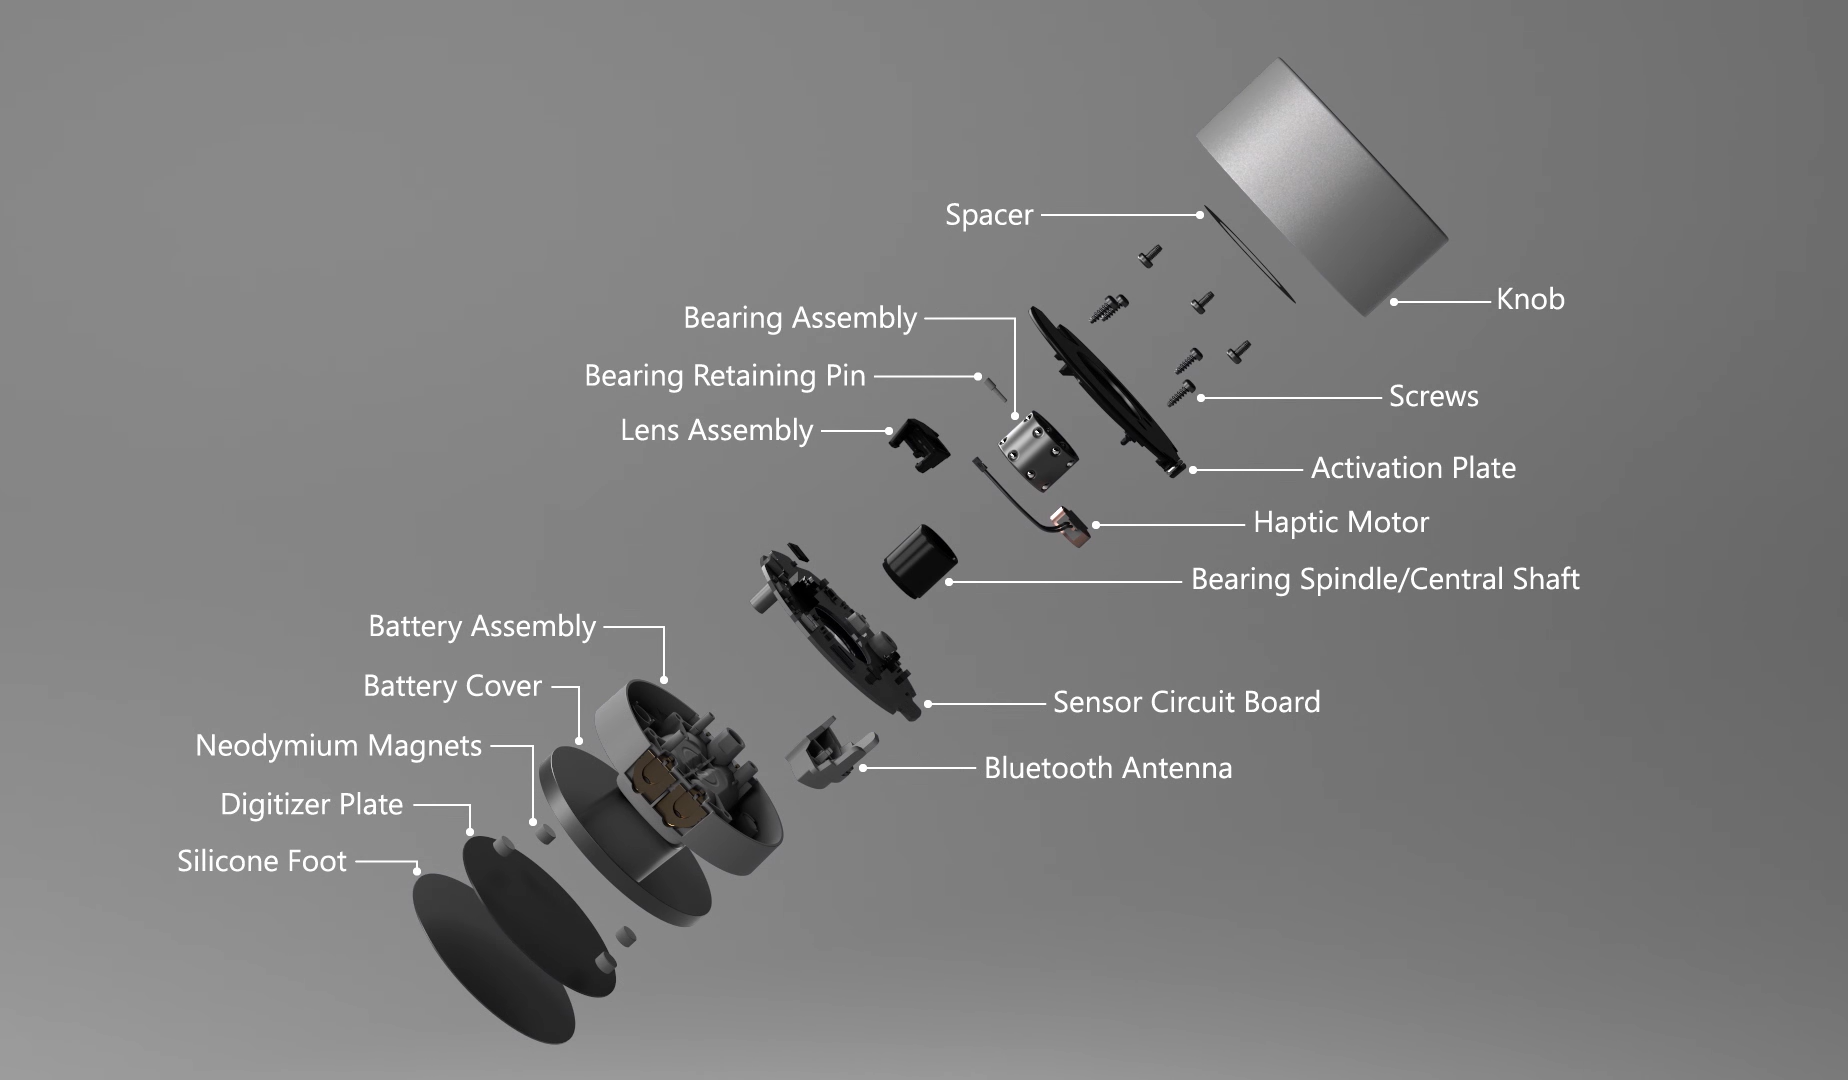
\includegraphics[width=0.9\textwidth]{DialEsploso}
		\caption{Dial Esploso}
    \end{minipage}
\end{figure}

Un ulteriore funzionalitá é rappresentata dal riconoscimento della posizione e del contatto del dispositivo con display touch-screen supportati, che avviene attraverso la presenza di quattro magneti al \emph{Neodymium}. 
\newpage
\subsection{Surface Pro 6}
\begin{figure}[htpb!]
\center
  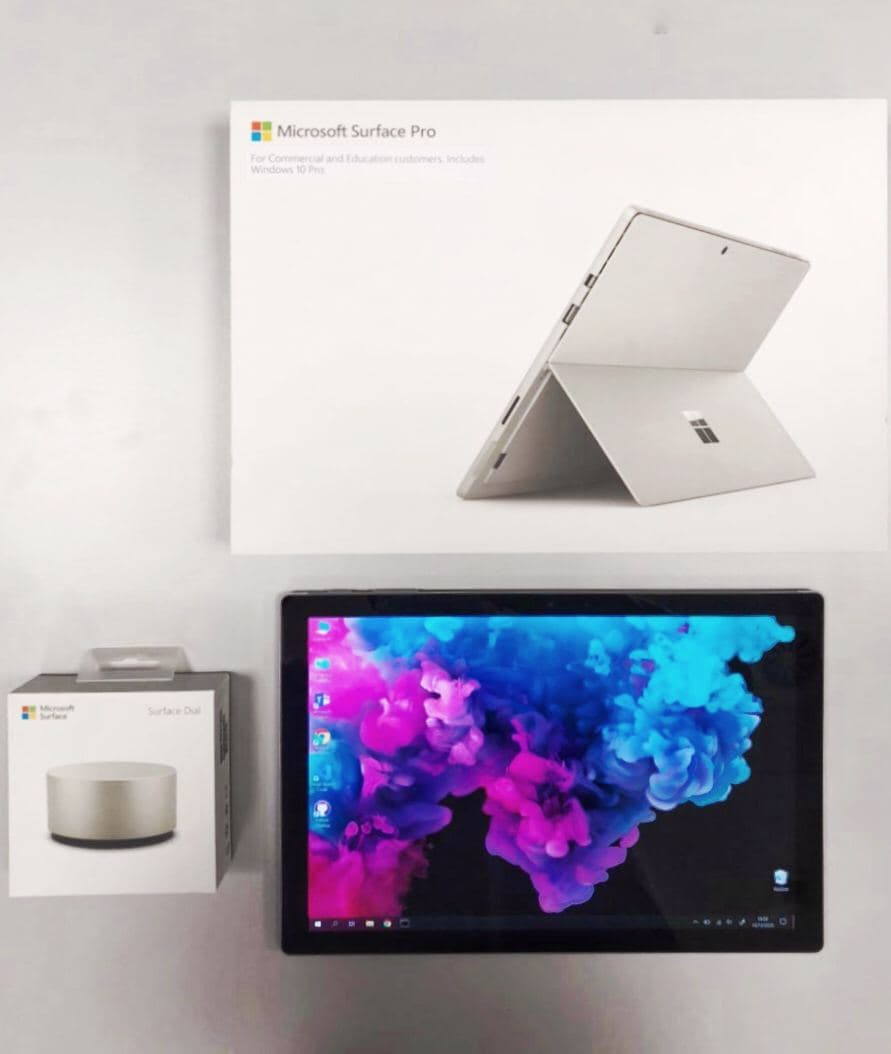
\includegraphics[width=0.3\textwidth]{Hardware}
  \caption{Surface Pro 6}
\end{figure}
Il Surface Pro 6\cite{sur} è un computer tablet 2-in-1 sviluppato da Microsoft . È la sesta generazione di Surface Pro ed è stato annunciato insieme al Surface Laptop 2 il 2 ottobre 2018 in un evento a New York.
\subsection{Aulos}
\begin{figure}[htpb!]
\center
  
\includegraphics[width=0.3\textwidth]{LogoAulos}
  \caption{Aulos}
\end{figure}
AULOS \cite{aul} è un framework ad uso interno per la standardizzazione dello sviluppo delle commesse.
Gli obiettivi principali di questo framework sono:
\begin{itemize}
\item rendere standard e subito disponibili quelle funzionalità che sono di frequente implementazione tra le commesse;
\item fornire uno standard UI e UX che sia ben riconoscibile, ma soprattutto coerente tra commesse diverse;
\item garantire l’interoperabilità tra tecnologie diverse.
\end{itemize}

AULOS fa uso di tecnologie web come Angular per il proprio frontend, mentre il backend – a cui esso si aggancia e che regola il funzionamento della commessa – può essere scritto in più linguaggi come C\# e LabView.
Da qui si nota come AULOS sia anche uno standard di comunicazione: l’utilizzo di API apre alla possibilità di sviluppare il backend nella tecnologia che meglio si sposa con il problema da risolvere.
\subsection{Angular}
\begin{figure}[htpb!]
\center
  
\includegraphics[width=0.2\textwidth]{LogoAngular}
  \caption{Angular}
\end{figure}
Angular 2+\cite{ang} (o semplicemente Angular) è un framework open source per lo sviluppo di applicazioni web con licenza MIT, evoluzione di AngularJS. Sviluppato principalmente da Google, la sua prima release è avvenuta il 14 settembre 2016.Angular è stato completamente riscritto rispetto a AngularJS e le due versioni non sono compatibili. Il linguaggio di programmazione usato per AngularJS è JavaScript mentre quello di Angular è TypeScript. Le applicazioni sviluppate in Angular vengono eseguite interamente dal web browser dopo essere state scaricate dal web server (elaborazione lato client). Questo comporta il risparmio di dover spedire indietro la pagina web al web-server ogni volta che c'è una richiesta di azione da parte dell'utente. Il codice generato da Angular gira su tutti i principali web browser moderni quali ad esempio Chrome, Microsoft Edge, Opera, Firefox, Safari ed altri. Angular è stato progettato per fornire uno strumento facile e veloce per sviluppare applicazioni che girano su qualunque piattaforma inclusi smartphone e tablet. Infatti le applicazioni web in Angular in combinazione con il toolkit open source Bootstrap diventano responsive, ossia il design del sito web si adatta in funzione alle dimensioni del dispositivo utilizzato. È in corso di sviluppo un altro toolkit di design responsivo, Flex Layout, più semplice da usare rispetto a Bootstrap e concepito appositamente per Angular. Altro toolkit che facilita la progettazione in Angular è Angular Material, una serie di componenti che permette di creare una pagina web molto velocemente: con l'utilizzo combinato di Flex Layout ed Angular Material si possono creare siti e applicazioni web responsive molto avanzate basate su Angular.
\subsection{TypeScript}
\begin{figure}[htpb!]
\center
  
\includegraphics[width=0.4\textwidth]{LogoTypescript}
  \caption{Typescript}
\end{figure}
TypeScript\cite{typ} è un linguaggio di programmazione open source sviluppato da Microsoft. Si tratta di un Super-set di JavaScript che basa le sue caratteristiche su ECMAScript 6; capo del progetto è Anders Hejlsberg. Il linguaggio estende la sintassi di JavaScript in modo che qualunque programma scritto in JavaScript sia anche in grado di
16
funzionare con TypeScript senza nessuna modifica. È stato progettato per lo sviluppo di grandi applicazioni ed è destinato a essere compilato in JavaScript per poter essere interpretato da qualunque web browser o app.
\subsection{HTML}
\begin{figure}[htpb!]
\center
  
\includegraphics[width=0.2\textwidth]{LogoHTML}
  \caption{HTML}
\end{figure}
L'HTML\cite{html} è un linguaggio di pubblico dominio, la cui sintassi è stabilita dal World Wide Web Consortium (W3C). È derivato dall'SGML, un metalinguaggio finalizzato alla definizione di linguaggi utilizzabili per la stesura di documenti destinati alla trasmissione in formato elettronico. La versione attuale, la quinta, è stata rilasciata dal W3C nell'ottobre 2014. Il motivo principale che ha spinto il W3C e i suoi membri a sviluppare HTML5 è stata la necessità di fornire direttamente le funzionalità che in precedenza erano fruibili tramite estensioni proprietarie all'esterno dei browser, come Adobe Flash e simili. Un secondo obiettivo che gli sviluppatori si erano prefissati era quello di garantire una maggiore compatibilità tra i diversi browser, indipendentemente dalla piattaforma software utilizzata, e principalmente mirata all'espansione dei dispositivi mobili.
\subsection{KendoUI}
\begin{figure}[htpb!]
\center
  
\includegraphics[width=0.3\textwidth]{LogoKendo}
  \caption{KendoUI}
\end{figure}
Kendo UI\cite{ken} e un framework integrale di interfaccia utente HTML5 per costruire applicazioni e siti web interattivi e ad alte prestazioni.
\subsection{Microsoft UWP}
\begin{figure}[htpb!]
\center
  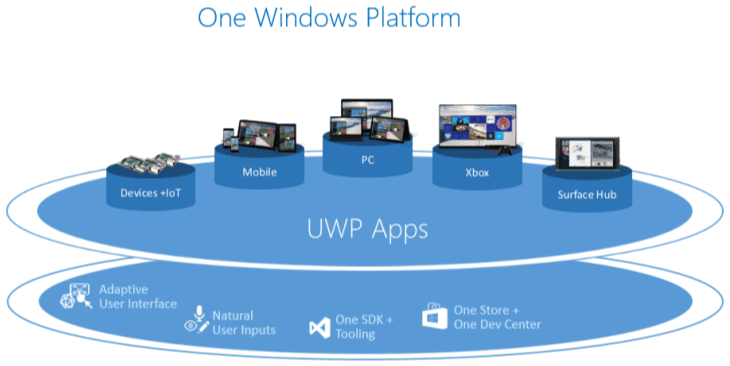
\includegraphics[width=0.45\textwidth]{LogoUWP}
  \caption{Microsoft UWP}
\end{figure}
UWP\cite{uwpdoc} è uno dei numerosi modi per creare applicazioni client per Windows. Le app UWP usano le API WinRT per offrire potenti funzionalità avanzate di interfaccia utente e asincrone, ideali per i dispositivi connessi a Internet.
Per scaricare gli strumenti necessari per iniziare a creare le app UWP, vedere Effettuare la configurazione e quindi Scrivere la prima app ed è la soluzione ideale per creare app che vengono eseguite nei dispositivi Windows 10 e possono essere combinate con altre piattaforme. Le app UWP possono usare le API Win32 e le classi .NET (vedere Set di API per le app UWP, DLL per le app UWP e .NET per le app UWP).Il progetto di sviluppo Microsoft continua a evolversi e, insieme a iniziative come WinUI, MSIX e Project Reunion, UWP rappresenta uno strumento potente per la creazione di app client.
Un'app UWP è:
\begin{itemize}
\item Sicura: le app UWP dichiarano le risorse del dispositivo e i dati a cui accedono. L'utente deve autorizzare tale accesso.
\item In grado di usare un'API comune in tutti i dispositivi che eseguono Windows 10.
\item In grado di usare funzionalità specifiche del dispositivo e di adattare l'interfaccia utente alle dimensioni, alle risoluzioni e ai DPI dello schermo di dispositivi diversi.
\item Disponibile nel Microsoft Store in tutti i dispositivi (o solo a quelli specificati) che eseguono Windows 10. Il Microsoft Store offre diversi modi per realizzare profitti con un'app.
\item In grado di essere installata e disinstallata senza rischio o danni per il computer.
\item Coinvolgente: è possibile usare riquadri animati, notifiche push e attività utente che interagiscono con Sequenza temporale di Windows e la funzionalità di ripristino della ricerca dal punto in cui è stata interrotta di Cortana per coinvolgere gli utenti.
\item Programmabile in C\#, C++, Visual Basic e Javascript. Per l'interfaccia utente usare WinUI, XAML, HTML o DirectX
\end{itemize}
\subsection{Microsoft WebView}
Una WebView\cite{webview} integra all'interno di un' applicazione una visualizzazione che esegue il rendering di contenuto web tramite il motore di rendering di Microsoft Edge nel quale possono comparire anche collegamenti ipertestuali funzionanti.
Metodi utilizzati:
\begin{itemize}
\item \emph{AddWebAllowedObject(String, Object)}\cite{awao} Permette di iniettare oggetti runtime nativi windows come parametri globali del documento all'interno della WebView
\item \emph{InvokeScriptAsync(String, IEnumerable<String>)}\cite{isa} Permette l'invio di script specifici alla pagina web caricata con argomenti specifici come azione asincrona. 
\end{itemize}

\subsection{C\#}
\begin{figure}[htpb!]
\center
  
\includegraphics[width=0.2\textwidth]{LogoC}
  \caption{C\#}
\end{figure}
Il C\#\cite{cs} è un linguaggio di programmazione orientato agli oggetti sviluppato da Microsoft all'interno dell'iniziativa .NET, e successivamente approvato come standard dalla ECMA (ECMA-334) e ISO (norma ISO/IEC 23270).
La sintassi e struttura del C\# prendono spunto da vari linguaggi nati precedentemente, in particolare Delphi, C++, Java e Visual Basic.
\subsection{Libreria RadialController}
La libreria RadialController\cite{rad} e le API correlate consentono di personalizzare sia il menù dei comandi integrato che l'esperienza di interazione supportata dall’ app.
Metodi utilizzati:
\begin{itemize}


\item RadialController.CreateForCurrentView()\\
Metodo statico che consente di ricevere un oggetto della classe RadialController creato appositamente per il contesto in cui gira l’applicazione (Dial utilizzato, versione del sistema operativo, tipo di hardware, ...)
\item .CreateFromIcon("Sample", icon)\\
Metodo che consente di creare un RadialControllerMenuItem ovvero un oggetto che inserito all’interno del menu verrà visualizzato e consentirà di svolgere un determinato comportamento quando selezionato.
\item .Menu.Items.
\begin{itemize}
\item Add(RadialControllerMenuItem item)
\item Inserisce il RadialControllerMenuItem all’interno del menu.
\item CreateFromKnownIcon(string displayText, RadialControllerMenuKnownIcon value)
\item Crea un oggetto di tipo RadialControllerMenuItem da un’icona già presente nella libreria.
\item CreateFromIcon(string displayText, RandomAccessStreamReference icon)
\item Crea un oggetto di tipo RadialControllerMenuItem da un’icona presente negli assets
\item CreateFromFontGlyph(string displayText, string glyph, string fontFamily)
\item Crea un oggetto di tipo RadialControllerMenuItem da un font installato nel sistema / inserito nell’app, e da un codice esadecimale ad esso associato
\end{itemize}
\end{itemize}
Eventi utilizzati:
\begin{itemize}
\item radialController.ButtonClicked\\
Evento che informa della pressione breve del dispositivo Dial.
\item radialController.ButtonPressed\\
Evento che informa della pressione prolungata del dispositivo Dial
\item radialController.RotationChanged\\
Evento che informa della rotazione del dispositivo Dial
\item .ScreenContactStarted\\
Evento che informa del posizionamento del Dial su schermo
\item .ScreenContactContinued\\
Evento che informa sull’utilizzo del Dial su schermo
\item .ScreenContactEnded\\
Evento che informa sulla fine del posizionamento su schermo
\end{itemize}
API correlate\\
RadialControllerConfiguration è una classe correlata alla classe RadialController e permette di configurare l’oggetto della medesima classe modificando le sue proprietà.\\
SetDefaultMenuItems consente di scegliere tra le voci di menù già predisposte dalla libreria quale inserire nel menù.

\newpage
\subsection{Git}
\begin{figure}[htpb!]
\center
  
\includegraphics[width=0.2\textwidth]{LogoGit}
  \caption{Git}
\end{figure}
Un sistema di controllo di versione\cite{git} distribuito o decentralizzato (o DVCS da Distributed Version Control System) è una tipologia di controllo di versione che permette di tenere traccia delle modifiche e delle versioni apportate al codice sorgente del software, senza la necessità di dover utilizzare un server centrale, come nei casi classici.

Con questo sistema gli sviluppatori possono collaborare individualmente e parallelamente non connessi su di un proprio ramo (branch) di sviluppo, registrare le proprie modifiche (commit) ed in seguito condividerle con altri o unirle (merge) a quelle di altri, il tutto senza bisogno del supporto di un server centralizzato. Questo sistema permette diverse modalità di collaborazione, proprio perché il server è soltanto un mero strumento d'appoggio.
\subsection{GitLab}
\begin{figure}[htpb!]
\center
  
\includegraphics[width=0.2\textwidth]{LogoGitLab}
  \caption{GitLab}
\end{figure}
GitLab\cite{gitl} è una piattaforma web open source che permette la gestione di repository Git e di funzioni trouble ticket. Appartiene a GitLab Inc.
Come tutti i software di controllo versione, GitLab permette la creazione di repository pubblici o privati, in cui gli sviluppatori possono caricare il proprio codice e gestire le modifiche alle varie
11
versioni in contemporanea al lavoro di più persone. In GitLab è possibile lavorare parallelamente ad altre persone sullo stesso progetto senza generare conflitti, caricare il proprio lavoro nel repository remoto (operazione di push) e poter unire alla fine le modifiche di tutti in un unico progetto (operazione di merge). È possibile fare delle merge request per il proprietario del repository, oltre al tracciamento degli issue, la possibilità di scrivere commenti e allegare documenti. GitLab mette a disposizione diverse funzionalità a seconda del tipo di abbonamento e del prezzo pagato. È comunque possibile utilizzarlo gratuitamente, seppur con delle limitazioni.

\newpage
\subsection{Miro}
\begin{figure}[htpb!]
\center
  
\includegraphics[width=0.3\textwidth]{LogoMiro}
  \caption{Miro}
\end{figure}
Miro\cite{miro} è la piattaforma di lavagna collaborativa online per il lavoro moderno, consentendo a team collocati, distribuiti e remoti di comunicare e collaborare tra formati, strumenti, canali e fusi orari, senza i vincoli di posizione fisica, spazio per riunioni e lavagna
\subsection{Teams}
\begin{figure}[htpb!]
\center
  
\includegraphics[width=0.4\textwidth]{LogoTeams}
  \caption{Teams}
\end{figure}
Microsoft Teams\cite{mt} è una piattaforma di comunicazione e collaborazione unificata che combina chat di lavoro persistente, teleconferenza, condivisione di contenuti (incluso lo scambio e il lavoro simultaneo sui file) e integrazione delle applicazioni. Il servizio si integra con la suite di produttività per l'ufficio in abbonamento di Microsoft 365 e include estensioni che possono integrarsi con prodotti non Microsoft.
\subsection{Trello}
\begin{figure}[htpb!]
\center
  
\includegraphics[width=0.2\textwidth]{LogoTrello}
  \caption{Trello}
\end{figure}
Trello\cite{tr} è un software gestionale in stile Kanban basato sul web che consente agli utenti la possibilità di creare le loro schede attività con più colonne e scambiare le attività tra di loro. In genere le colonne sono organizzate in stati dell'attività: Da fare, In corso, Fatto. Il software è utilizzabile per uso personale e aziendale. Ha una varietà di possibilità di impiego, come la gestione immobiliare, la gestione di progetti software, i bollettini scolastici, la pianificazione delle lezioni, la contabilità, il web design, i giochi e la gestione di casi legali.

\newpage
\subsection{Visual Studio}
\begin{figure}[htpb!]
\center
  
\includegraphics[width=0.2\textwidth]{LogoVS}
  \caption{Visual Studio}
\end{figure}
Microsoft Visual Studio\cite{vs} (o più comunemente Visual Studio) è un ambiente di sviluppo integrato (Integrated development environment o IDE) sviluppato da Microsoft.
Visual Studio è multilinguaggio e attualmente supporta la creazione di progetti per varie piattaforme, tra cui anche Mobile e Console. È possibile creare ed utilizzare estensioni e componenti aggiuntivi.
Visual Studio, nelle sue ultime versioni da quando è nata la piattaforma .NET, supporta diversi linguaggi di programmazione tra cui C\#, Visual Basic .Net e C++. Nelle passate edizioni era disponibile anche il supporto a J\#. Visual Studio è incompatibile col linguaggio Java da cui comunque il linguaggio J\# aveva preso forte ispirazione.
Come il suo predecessore, Visual Studio integra la tecnologia IntelliSense che permette di correggere eventuali errori sintattici, e anche alcuni logici, senza compilare l'applicazione, possiede un debugger interno per il rilevamento e la correzione degli errori logici nel codice in runtime e fornisce diversi strumenti per l'analisi delle prestazioni.Si integra nativamente con l'ambiente di sviluppo di gruppo Team Foundation Server che, tra le altre cose, permette di effettuare operazioni di versioning del codice.
Visual Studio dispone di diversi template per ciascun linguaggio di programmazione supportato, ad esempio Applicazione desktop, libreria di classi, servizio di Windows e diversi sottomenu che consentono di indirizzarsi sulla piattaforma per cui si desidera sviluppare. Tra queste: Microsoft Azure, Windows Store e smartphone Android e iOS
17
grazie all'integrazione con Xamarin. Le applicazioni desktop in Visual Basic .NET e Visual C\# possono essere a loro volta sviluppate utilizzando la classica tecnologia dei form oppure Windows Presentation Foundation.Nelle due versioni 2015 e 2017 il programma si è notevolmente ingrandito fino a una dimensione di circa 80 GB per un'installazione completa. Infatti sono state introdotte nuove funzioni come il supporto per gli strumenti nativi Python e applicazioni Linux, l'integrazione con Unity per lo sviluppo di videogiochi, il simulatore Android e iOS, la possibilità di gestire e modificare cursori, icone e immagini all'interno dell'applicazione.
L'interfaccia grafica dell'IDE dispone di una casella degli strumenti, disponibile solo per VB.NET, C\# e ASP.NET, da cui è possibile trascinare i controlli (tra cui TextBox, Label, ImageBox, Button) direttamente nel form del programma che si sta progettando e modificarne l'aspetto senza necessariamente passare dal codice. Attraverso gli eventi si gestisce il comportamento di questi componenti.Inoltre Visual Studio consente di reperire e installare template e componenti aggiuntivi di terze parti dal Web per ottenere ulteriori funzionalità. Per esempio esistono estensioni che introducono il supporto per il linguaggio PHP.
\subsection{Remote Tools}
Remote Tool\cite{rd} è uno strumento messo a disposizione da Microsoft che permette il debug di applicazioni UWP su dispositivi remoti collegati all'interno della rete corrente.
\subsection{Visual Studio Code}
\begin{figure}[htpb!]
\center
  
\includegraphics[width=0.4\textwidth]{LogoVSCode}
  \caption{Visual Studio Code}
\end{figure}
Visual Studio Code\cite{vsc} è un editor di codice sorgente sviluppato da Microsoft per Windows, Linux e macOS. Include il supporto per debugging, un controllo per Git integrato, Syntax highlighting, IntelliSense, Snippet e refactoring del codice. Sono personalizzabili il tema dell'editor, le scorciatoie da tastiera e le preferenze. È un software libero e gratuito, anche se la versione ufficiale è sotto una licenza proprietaria.Visual Studio Code è basato su Electron, un framework con cui è possibile sviluppare applicazioni Node.js.
Visual Studio Code è un editor di codice sorgente che può essere usato con vari linguaggi di programmazione, tra cui la famiglia di linguaggi C (C, C++, C\#), F\#, HTML e altri linguaggi web, tra cui PHP, Java, Ruby e molti altri. Incorpora un insieme di funzioni che variano a seconda del linguaggio che si sta usando, come mostrato nella tabella seguente. Molte delle funzioni di Visual Studio Code non sono accessibili attraverso menu o interfacce utente, ma piuttosto attraverso una finestra di comando o un file .json, ad esempio le preferenze dell'utente. La finestra di comando è un'Interfaccia a riga di comando, che scompare appena l'utente clicca in un'area al di fuori della finestra o preme una serie di tasti per interagire con qualcosa al di fuori di essa.
In quanto editor di codice sorgente, Visual Studio Code permette la modifica della Codifica di caratteri, il carattere inizio nuova linea (si può scegliere tra LF e CR+LF) e il linguaggio di programmazione del documento che si sta modificando.

\chapter{Servizio}
\label{chap:serv}
In questo capitolo verranno esposti in dettaglio l'architettura finale dell'applicativo sviluppato che permette la comunicazione tra il Surface Dial e la pagina web, le funzionalitá implementate grazie al suddetto servizio, una breve descrizione per lo sviluppatore che intederá utilizzarlo e i test implementati attraverso MSTest con lo scopo di verificare il corretto funzionamento del software
\section{Architettura Software}
Il progetto sviluppato si presenta suddiviso in due parti ben distinte:
\begin{itemize}
\item \textbf{Servizio Angular}
\item \textbf{Applicazione UWP}
\end{itemize}

\subsection{Servizio Angular}

In Angular, i Servizi rappresentano un tassello fondamentale per la realizzazione di un'applicazione. Un servizio è solitamente rappresentato da una classe indipendente dalla View che viene definita per svolgere un compito ben preciso ed effettuare delle operazioni strettamente correlate tenendo in mente il principio di singola responsabilità.\\
È possibile definire più servizi all'interno di un'applicazione, ognuno dei quali si occupa di portare a termine un determinato incarico incrementando la modularitá del progetto, inoltre un servizio puó a sua volta dipendere da altri servizi, che vengono definiti nel costruttore del servizio stesso.\\

Avvalendosi di Angular CLI, possiamo creare un Servizio tramite il comando:

\vspace{1.0cm}
\begin{lstlisting}[caption={Esempio creazione servizio},style=javaScriptCode]
	ng generate service <nome-del-servizio> <flag-opzionali>
\end{lstlisting} 
\vspace{1.0cm}
Una volta creati, i servizi possono essere iniettati all'interno di uno o più componenti grazie al meccanismo di \emph{Dependency Injection}.\\

Per poter utilizzare un servizio da noi definito, dobbiamo registrarlo con uno degli Injector presenti in Angular. Esiste infatti una gerarchia di Injector, che Angular provvede a creare, alla base dei quali c'è il cosiddetto Root Injector, che viene creato in fase di bootstrap dell’applicazione e i servizi registrati con quest’ultimo sono disponibili per tutta l’applicazione.\\

Per ogni Injector esiste sempre una sola istanza di un determinato servizio, come specificato nella documentazione ufficiale:\\

\emph{"Services are singletons within the scope of an injector. That is, there is at most one instance of a service in a given injector."}\\

L’ Injector si occupa di creare le dipendenze e si serve di un Provider, un oggetto il quale indica all'Injector come ottenere o creare un'istanza di una dipendenza.
Per ogni dipendenza che si vuole usare nell'applicazione si deve registrare un provider con un Injector, in modo che quest'ultimo possa poi utilizzare il provider per creare nuova istanza di quella dipendenza.

\subsubsection{Singleton services}

Per restare in linea con le direttive utilizzare dal gruppo Loccioni nello sviluppo dei loro servizi, abbiamo utilizzato il forRoot() pattern per l’injection del servizio nell’applicazione.\\

Questo pattern permette di specificare un modulo personalizzato per il servizio, il quale contiene un metodo statico chiamato appunto forRoot() che restituisce un ModuleWithProvider parametrizzato al modulo del Servizio.\\

Questo pattern permette di effettuare l’import del modulo nell’AppModule richiamando il metodo forRoot(), cosi da non dover appesantire il Provider del modulo iniziale e in linea di principio é bene utilizzarlo quando un provider prende in ingresso dei parametri, così da non dover specificarli ogni qualvolta il modulo venga utilizzato.

\subsubsection{DialService}

Lo scopo finale del servizio che abbiamo implementato é quello di poterlo utilizzare come ponte o intermediario tra il Surface Dial, che si interfaccia nativamente con l'applicazione UWP, la quale contiene una WebView con all'interno caricata una pagina custom Loccioni, e i componenti della View all'interno della pagina che intendono utilizzare il servizio.\\

Il componente che dipenderá da questo determinato servizio, chiamato appunto DialService, potrá facilmente utilizzare le funzionalitá messe a disposizione dal Surface Dial e interpretare gli eventi intercettati a RunTime.\\

Il core del servizio implementato è rappresentato dalla Classe DialService, essa infatti si occupa di inizializzare il servizio e rendere disponibile la comunicazione bi-direzionale tra il lato Web e quello UWP.In particolare si occupa di recuperare l'oggetto C\# iniettato a sua volta dentro l'oggetto window della pagina web, con visibilitá globale.\\

\vspace{1.0cm}
\begin{lstlisting}[caption={Recupero oggetto C\#},style=javaScriptCode]
	this.dial = (window as any).dial;
\end{lstlisting} 
\vspace{1.0cm}

L'oggetto dial viene poi inserito per questioni di sicurezza in una classe DialProxy, la quale implementa a sua volta l'interfaccia da noi sviluppata DialBackendBridge, nella quale sono presenti tutte le funzionalitá dell'oggetto "dial", richiamabili quindi da Web.

\subsubsection{DialBackendBridge}

DialBeckendBridge rappresenta l'interfaccia contenente la dichiarazione dei metodi implementati nella classe DialController dell'applicazione UWP.\\
In questo modo, tramite l'oggetto dial iniettato, sará possibile richiamare a RunTime i metodi dichiarati nel C\# attraverso il Web.\\

\vspace{1.0cm}
\begin{lstlisting}[caption={Interfaccia DialBackendBridge},style=javaScriptCode]
export interface DialBackednBridge{
		
	getProductId(): string;
	
	setMenu(arrayOfItem: any[]): void;
	
	clearMenu(): void;
	
	deleteItem(tag: string): void;
	
	addItem(item: any): void;
	
	createDialMenuItem(tag: string, displayText: string, icon: string): any;
	
	setDefaultItem(defaultItems: string[]): void;
	
	manualInvoke(tag: string): void;		

}		
\end{lstlisting} 
\vspace{1.0cm}

\newpage
\subsubsection{DialFrontendBridge}

Per rendere questa comunicazione bi-direzionale, abbiamo creato una classe DialFrontendBridge con la responsabilitá di rendere visibili dei metodi all'interno dell'oggetto window e quindi richiamabili tramite script dall'applicazione UWP.\\

L'invocazione di questi metodi comporta la successiva emissione di un determinato evento a coloro che vi si sottoscrivono, con la possibilitá del passaggio di parametri di tipo stringa.\\

Tramite l'utilizzo degli EventEmitter messi a disposizione dal core di Angular e definiti come mostrato nel codice sottostante, la classe DialFrontendBridge permette all'utilizzatore del servizio di sottoscriversi a determinati eventi pubblici, che quando richiamati emettono un determinato valore.\\

\vspace{1.0cm}
\begin{lstlisting}[caption={EventEmitter esposti da DialFrontendBridge},style=javaScriptCode]
public onRotationEvent = new EventEmitter<{tag: string, degree: string}>();
public onPressedRotationEvent = new EventEmitter<{tag: string, degree: string}>();
public onClickEvent = new EventEmitter<string>();
public onInvokeEvent = new EventEmitter<string>();
public onScreenContactStartedEvent = new EventEmitter<{x: string, y: string}>();
public onScreenContactContinuedEvent = new EventEmitter<{x: string, y: string}>();
public onScreenContactEndedEvent = new EventEmitter();
\end{lstlisting} 
\vspace{1.0cm}

Affinché questi metodi possano essere richiamati tramite script dall'applicazione UWP é stato necessario inserire l'istanza della classe all'interno dell'oggetto window, cosi da renderlo visibile e utilizzabile dall'esterno.\\

\vspace{1.0cm}
\begin{lstlisting}[caption={Inserimento DialFrontendbridge in window },style=javaScriptCode]
(windowa as any).DialFrontendBridge = this.dialFrontendbridge;
\end{lstlisting} 
\vspace{1.0cm}

\newpage
\vspace{1.0cm}
\begin{lstlisting}[caption={Metodi esposti DialFrontendBridge},style=javaScriptCode]
    public RotationEvent(tag: string, degree: string): string{
        this.onRotationEvent.emit({tag, degree});
        return degree;
    }
    public PressedRotationEvent(tag: string, degree: string): string{
        this.onPressedRotationEvent.emit({tag, degree});
        return degree;
    }
    public ClickEvent(tag: string){
            this.onClickEvent.emit(tag);
    }
    public InvokeEvent(tag: string){
        this.onInvokeEvent.emit(tag);
    }
    public ScreenContactStartedEvent(x: string, y: string){
        this.onScreenContactStartedEvent.emit({x, y});
    }
    public ScreenContactContinuedEvent(x: string, y: string){
        this.onScreenContactContinuedEvent.emit({x, y});
    }
    public ScreenContactEndedEvent(){
        this.onScreenContactEndedEvent.emit();
    }
\end{lstlisting} 

\subsubsection{Widget}

TODO: DA COMPLETARE

Un widget Aulos è un componente in esecuzione all’interno di una DashBoard con lo scopo di rappresentare o modificare i dati ottenuti dal backend collegato fisicamente ad una macchina.\\

Nella nostra applicazione abbiamo modificato degli Widgets giá esistenti, utilizzando all'interno di essi il nostro servizio \emph{DialService}, allo scopo di renderli controllabili attraverso il Dial.Siamo partiti tentando di agganciarsi ad un semplice Widget che visualizza un range di possibili valori rappresentato da uno \emph{slider grafico}, con l'intento di variare, anche solo graficamente, il valore corrente attraverso l'evento rotazione del Dial.\\

\begin{lstlisting}[caption={Sottoscrizione evento rotazione},style=javaScriptCode]
if (this.widget.runMode){
  if (this.dialService.isDialConnected){
	this.createMenuVoice();
	this.dialService.dialFrontendBridge.onRotationEvent.subscribe(
	({tag, degree}) => {
	  if (tag === this.id){
		this.value += (parseInt(degree, 10) * 5);
		this.changeDetectorRef.detectChanges();
	  }
	});
  }
}
\end{lstlisting} 

La stessa cosa è stata fatta per un widget rappresentato graficamente da un \emph{Radial Gauge}, fino ad arrivare a modificare valori lato Backend attraverso il DialChannelWidget, un widget creato da noi che contiene al suo interno , al contrario degli widget già presenti, il collegamento a \emph{N} diversi canali modificabili.
Questo ci ha permesso di sviluppare delle funzionalità custom per quel determinato Widget al fine di poterne acquisire il controllo, e scegliere canale per canale, il valore da settare, permettendo la variazione non solo grafica ma anche effettiva dei dati mostrati.\\

Per rendere sicura queste funzionalità abbiamo previsto la variazione dei valori con la singola rotazione e la successiva modifica lato backend qualora il dial venga premuto, altrimenti attraverso la funzionalità combinata di pressione e rotazione, così da evitare una involontaria modifica nel momento della presa possesso.\\

Analogamente all'evento sopra mostrato, chiamato onRotationEvent, gli eventi al quale il widget ChannelDialWidget si sottoscrive al fine di variare i valori di un canale selezionato, sia graficamente che in modo permanente lato backend, sono i seguenti:

\begin{itemize}
\item \textbf{onRotationEvent} 
\item \textbf{onClickEvent} 
\item \textbf{onPressedRotationEvent}
\end{itemize}

Durante la sua inizializzazione, il widget si sottoscrive all'evento di Invoke, con lo scopo di intercettare il tag sul quale viene richiamato il medesimo metodo dal Dial. Successivamente, se l'invoke richiamato restituisce il tag corrispondente all'ID del Widget in ascolto, viene pulito il menu del dial e vengono caricate le voci di menu inerenti ai canali collegati a quel determinato Widget cosi da poter essere richiamati e intercettati a loro volta dalla sottoscrizione all'evento onInvokeEvent.
 
\subsection{Applicazione UWP}

La seconda parte, invece, è costituita da un’ applicazione UWP ovvero Universal Windows Platform, presa in considerazione poiché la più recente tra i framework Microsoft e tra le sue caratteristiche troviamo la sicurezza e la portabilità tra le diverse piattaforme windows, ciò consente un maggiore supporto nel tempo e intercambiabilità tra i dispositivi dove utilizzarla.\\

L’applicazione DialBridge ha come responsabilità quella di comunicare con il Dispositivo HID attraverso le librerie fornite da Microsoft e allo stesso tempo comunicare con la pagina Web contenuta al suo interno.\\

Inizialmente abbiamo creato un’unica soluzione contenente sia la Web View che il Core dell’applicazione, ma abbiamo riscontrato un problema nell’injection dell’oggetto utilizzato per la comunicazione Web-UWP, poichè esso deve necessariamente essere iniettato a runtime.\\

Di conseguenza abbiamo creato due diverse soluzioni:

\begin{itemize}
\item \textbf{Core:} Contiene il nucleo dell’applicazione.
\item \textbf{EmbeddedBrowserView:} Contiene la parte runtime del progetto e effettua l’injection dell’oggetto nella pagina Web.
\end{itemize}

\subsubsection{Core}

Nel Core è contenuta la parte del progetto UWP che non richiede la partenza a runtime e comprende le seguenti classi:

\begin{itemize}
\item AulosCollection
\item AulosIcon
\item DialController
\item WebNotifier
\item DialMenuItem
\end{itemize}

\subsubsection{AulosCollection e AulosIcon}

Queste due classi si occupano, insieme al main, della parte riguardante le icone che verranno poi visualizzate nel menu del Dial. All’avvio dell’applicazione nella classe main viene effettuata una chiamata GET ad un eventuale server Loccioni che consente di ricevere un file JSON contenente una mappa “nome”-”FontGlyph” che verrà poi utilizzato per creare un DialMenuItem insieme al Font Aulos creato da Loccioni.\\

L’utilizzo di questo approccio consente una maggiore facilità nella sostituzione delle icone, che non dipende dalle risorse dell’applicazione stessa ma da un server Loccioni.

\subsubsection{DialController}

La classe DialController è una tra le più importanti poiché una sua istanza verrà poi inserita all’interno della WebView e servirà al servizio DialService per la comunicazione Web-UWP. I metodi pubblici al suo interno sono gli stessi dell’interfaccia DialBackendBridge che vengono utilizzati appunto tramite l’oggetto iniettato inizialmente.\\

Al suo interno troviamo un’ istanza della classe RadialController, ovvero la libreria Microsoft che permette la manipolazione del Dial, un'istanza di RadialControllerConfiguration e infine un notifier.\\

Nel costruttore abbiamo assegnato agli eventi presenti nella classe RadialController il relativo handler nella classe WebNotifier, in questo modo ogni volta che verrà emesso un determinato evento la pagina web riceverà una notifica e verrà svolta la funzione associata a quella determinata voce di menù.

\subsubsection{WebNotifier}

La classe WebNotifier contiene al suo interno una istanza della WebView ed ha come responsabilità quella di fornire i metodi che verranno poi utilizzati come EventHandler per gli eventi forniti dalla classe RadialController, in modo tale da riuscire a comunicare, attraverso la WebView al suo interno, alla pagina web l’emissione dell’evento stesso.\\

Al suo interno è presente anche un oggetto della classe CoreWindow utilizzato per spostare la posizione del mouse sullo schermo al primo contatto del Dial sulla superficie.

\subsubsection{DialMenuItem}

La classe DialMenuItem è una classe “modello” utilizzata per rappresentare un elemento contenuto nel Menu del Dial.

\subsubsection{MainPage}

Nella Main Page avviene l’inizializzazione dei componenti RadialController e la navigazione alla pagina web desiderata.\\

All’interno del metodo NavigationStarting troviamo il metodo AddWebAllowedObject che ci permette, una volta caricata la pagina, di iniettare l’oggetto della classe DialController per la comunicazione.

\section{Funzionalità implementate}

\subsection{Aquisizione widget}
\subsection{Posizionamento su schermo}

Uno dei maggiori vantaggi dell’utilizzo di un surface Dial è la possibilità di posizionarlo sopra uno schermo compatibile e di cambiare il suo funzionamento in base alla posizione utilizzata.
Questa funzionalità è gestita dal sistema operativo e comunica solamente con elementi nativi UWP, considerando ciò, abbiamo cercato un servizio Angular che ci permettesse di svolgere la stessa funzione all’interno di una pagina web ma senza risultati.
\begin{figure}[htpb!]
  \centering
  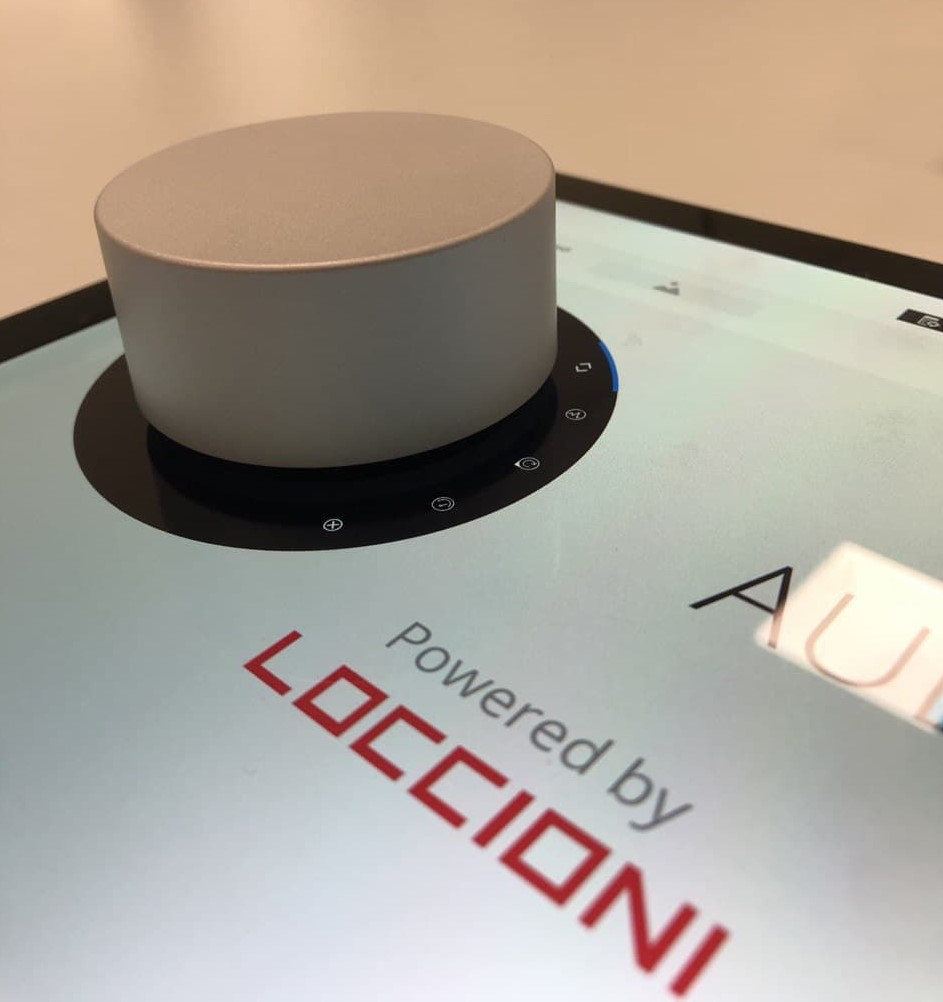
\includegraphics[width=0.5\textwidth]{DialSchermo}
  \caption{Microsoft Dial posizionato sopra un surface pro 6}
\end{figure}
Inizialmente abbiamo preso in considerazione la possibilitá di suddividere il layout dell’applicazione nativa in N riquadri, all’interno dei quali avremo posizionato il relativo Widget da controllare. Questa soluzione presenta peró delle limitazioni, in quanto in base alla risoluzione del dispositivo utilizzato, i widget caricabili in ogni riquadro del layout erano limitati al numero di riquadri definiti dall’applicazione UWP.

Abbiamo quindi cercato una soluzione, che spostasse la responsabilitá di acquisire il posizionamento lato Web anziché lato UWP. Dopo vari tentativi, abbiamo escogitato una soluzione che ci permettesse di avere un numero variabile di Widget configurabili nella Dashboard e la successiva acquisizione di essi, per fare ciò abbiamo sfruttato
Analizzando gli eventi richiamabili dalla classe RadialController, in particolare quelli inerenti al contatto con lo schermo, abbiamo notato prendevano in ingresso un oggetto di tipo RadialControllerScreenContact fornitogli dalla Libreria. Questo oggetto possiede due attributi relativi al Posizionamento ( Position ) e al Bound ( Bounds ) del rettangolo generato dal Dial sullo schermo.

Grazie all’attributo Position di tipo Point, é possibile ottenere, attraverso le coordinate X e Y, il punto centrale nel quale il Dial é posizionato.

\vspace{1.0cm}
\begin{lstlisting}[caption={Metodo ScreenContactStartedAsync},style=javaScriptCode]
 internal async Task ScreenContactStartedAsync(
 	RadialControllerScreenContactStartedEventArgs args
 )
  {
    this.simpleHaptics = args.SimpleHapticsController;
    string x = args.Contact.Position.X.ToString();
    string y = args.Contact.Position.Y.ToString();
    window.PointerPosition = new Point(
    	args.Contact.Position.X, 
    	args.Contact.Position.Y
    	);
    string function = 
    "window.DialFrontendBridge.ScreenContactStartedEvent('" + x + "', '" + y + "')";
    await webView.InvokeScriptAsync("eval", new string[] { function });
    onScreen = true;
    inputInjector.InjectMouseInput(new[] { inputInfo });
    inputInfo.MouseOptions = InjectedInputMouseOptions.Move;
    inputInfo.DeltaY = 1;
  }
\end{lstlisting} 
\vspace{1.0cm}


Attraverso la libreria Window.UI.Core é possibile spostare il cursore in un punto definito della UI corrente. Per questo motivo, la classe WebNotifier presente un attributo private e readonly chiamato window, un oggetto di tipo WindowCore che permette di intercettare eventi relativi ai dispositivi di Input utilizzati ma anche di posizionare il cursore del dispositivo in una posizione specifica in base alle coordinate passategli. In questo modo, attraverso l’attributo PointerPosition siamo stato in grado di creare un nuovo oggetto di tipo Point con le coordinate X e Y acquisite dal Dial consentendoci di posizionare il cursore in quel determinato punto.
\vspace{1.0cm}
\begin{lstlisting}[caption={Spostamento cursore},style=javaScriptCode]
  window.PointerPosition = new Point(args.Contact.Position.X, args.Contact.Position.Y);
\end{lstlisting} 
\vspace{1.0cm}
Questa soluzione ci ha permesso di spostare dinamicamente il cursore nella posizione centrale al disotto del Dial quando viene posizionato sopra lo schermo così da poter intercettare lato Web la posizione del cursore e permettere agli utilizzatori del servizio di riprodurre il comportamente appropriato per il Widget sopra il quale ci si posiziona.
Abbiamo quindi previsto nel Template HTML del Widget un metodo OnMouseOver che venisse richiamato solamente qualora il Dial fosse effettivamente a contatto con lo schermo, ma il semplice spostamento del cursore nella nuova posizione non richiamava correttamente il metodo in quanto il cursore non effettuava un movimento, ma veniva ricreato in quella determinata posizione.
Affinché la soluzione ideata funzionasse correttamente abbiamo importato una libreria chiamata Windows.UI.Input.Preview.Injection che mette a disposizione funziolitá per la simulazione di eventi di input.

Una volta posizionato il cursore nella nuova posizione, siamo stati in grado di simulare un impercettibile movimento del cursore di un singolo pixel, grazie al quale ci é stato possibile intercettare correttamente l’evento OnMouseMove dichiarato nel Template del Widget eseguendo il metodo associato.

\vspace{1.0cm}
\begin{lstlisting}[caption={Spostamento cursore},style=javaScriptCode]
inputInjector.InjectMouseInput(new[] { inputInfo });
inputInfo.MouseOptions = InjectedInputMouseOptions.Move;
inputInfo.DeltaY = 1;
\end{lstlisting} 
\vspace{1.0cm}
\subsection{Feedback aptico}
\subsection{Variazione degree personalizzata}
\section{Utilizzo del Servizio}

Per utilizzare il servizio DialService, occorre importarlo nel costruttore del componente che si sta sviluppando, in questo modo avremo accesso agli eventi che ci consentono di avere notifiche dal Dial.
Inizialmente è necessario creare una voce di Menù che rappresenta il widget all’interno del menù del Dial, così da avere la possibilità di acquisirne il controllo ed avere accesso alle sue funzionalità.
Sotto è riportato un esempio di creazione di una voce di menù per il dial con la relativa aggiunta alla lista di voci di Menu giá presenti.

\vspace{1.0cm}
\begin{lstlisting}[caption={Creazione nuova voce da widget},style=javaScriptCode]
  private createMenuVoice() {
    const dialMenuVoice = this.dialService.dialProxy.createDialMenuItem(
      this.widget.id, this.widget.descriptor.shortText, this.widget.descriptor.icon);
    this.dialService.dialProxy.addItem(dialMenuVoice);
  }
\end{lstlisting} 
\vspace{1.0cm}

Una volta aggiunta la voce di Menu al Dial, essa potrá essere selezionata attraverso il metodo Inkove messo a disposizione dalla classe DialController. Il metodo Invoke per acquisire una voce di menu, potrá essere richiamato sia attraverso il menu contestuale del Dial che compare nello schermo, che tramite un nostro metodo chiamato appunto ManualInvoke che esegue questa azione manualmente, richiamando tramite Web il medesimo metodo, solamente se quella voce di menu é presente tra quelle disponibile nel Dial.
In questo modo, il Widget non dovrá fare altro che mettersi in ascolto del metodo onInvokeEvent, il quale quando richiamato, restituisce una stringa definita “tag”, rappresentante la voce Menu acquisita.
Se quel tag, corrisponde all’id del Widget in ascolto, significa che l’utente ha richiesto il controllo di quel determinato Widget.

\vspace{1.0cm}
\begin{lstlisting}[caption={Ascolto Invoke della voce di menu'},style=javaScriptCode]
  this.dialService.dialFrontendBridge.onInvokeEvent.subscribe(tag => {
        if (tag === this.widget.id) {
          this.isActive = true;
          this.dialService.widget = this.widget.id;
          this.widgetDialStart();
          this.dialService.dialProxy.manualInvoke(this.channels[0].parameter.value);
        }
\end{lstlisting} 
\vspace{1.0cm}

Una volta acquisito il controllo del Widget, bisognerá mettersi in ascolto delle funzioni richiamabili dal Dial, attraverso gli eventEmitter messi a disposizione dalla classe DialFrontndBridge, e implementare il comportamento di quel Widget all’emissione di determinati eventi come la Rotazione o il Click.


\vspace{1.0cm}
\begin{lstlisting}[caption={Ascolto eventi associati alla voce di menu' selezionata},style=javaScriptCode]
const rotation = this.dialService.dialFrontendBridge.onRotationEvent.subscribe(
	({ tag, degree }) => {
      // Azione associata all'evento rotazione del Dial.
      if (tag === this.channels[this.currentChannel].parameter.value) {
        this.setSetterAtIndex(this.currentChannel, 
        parseNumber(degree)* this.moltiplicator
        );
      }
    });

const click = this.dialService.dialFrontendBridge.onClickEvent.subscribe(
	(tag) => {
      // Azione associata all'evento click del Dial.
      if(tag === this.channels[this.currentChannel].parameter.value){
          this.setChannelValue(this.channels[this.currentChannel].parameter.code,
          this.getNumberSetterComponent(this.currentChannel).value);
        }
    });

const pressRot = this.dialService.dialFrontendBridge.onPressedRotationEvent.subscribe(
({ tag, degree }) => {
      // Azione associata all'evento rotazione con pressione del Dial.
      if (tag === this.channels[this.currentChannel].parameter.value) {
        this.setSetterAtIndex(
        this.currentChannel, 
        parseNumber(degree) * this.moltiplicator
        );
        this.setChannelValue(this.channels[this.currentChannel].parameter.code,
        this.getNumberSetterComponent(this.currentChannel).value);
      }
    });
    this.channelDialSubscriptions?.unsubscribe();
    this.channelDialSubscriptions = new Subscription();
    this.channelDialSubscriptions.add(rotation).add(click).add(pressRot);
\end{lstlisting} 
\vspace{1.0cm}


I metodo sopra implementati, permettono di eseguire una determinata azione quando viene richiamato un metodo presente in DialFrontendBridge come la rotazione o la pressione combinata alla rotazione, che permette quindi nel caso dell'acquisizione tramite il contatto del Dial sullo schermo, mantenendo il controllo e il relativo comportamento, anche appoggiandolo sulla scrivania, evitano il pericolo che nel tratto in cui é il dispositivo si trova sospeso, possano avvenire chiamate pericolose.

\section{Testing}

Per quanto riguarda i test svolti in ambito UWP abbiamo utilizzato MSTest fornito da Microsoft all’interno di Visual Studio per testare le funzionalitá messe a disposizione dalla classe RadialController.

\subsection{MSTest}
Visual Studio Unit Testing Framework descrive la suite di strumenti di unit test di Microsoft integrata in alcune versioni di Visual Studio 2005 e successive.
Qui sotto sono riportati due tra i vari test implementati nel progetto:
 
\vspace{1.0cm}
\begin{lstlisting}[caption={Test SetMenu},style=javaScriptCode]
    [UITestMethod]
        public void TestSetMenu()
        {
            Assert.IsFalse(radialController.Menu.Items.Count > 0);
            DialMenuItem item1 = dialController.CreateDialMenuItem("tag1", "d", "icon");
            DialMenuItem item2 = dialController.CreateDialMenuItem("tag2", "d", "icon");
            DialMenuItem item3 = dialController.CreateDialMenuItem("tag3", "d", "icon");
            DialMenuItem item4 = dialController.CreateDialMenuItem("tag4", "d", "icon");
            List<DialMenuItem> items = new List<DialMenuItem>();
            items.Add(item1);
            items.Add(item2);
            items.Add(item3);
            items.Add(item4);
            dialController.SetMenu(items);
            Assert.IsTrue(radialController.Menu.Items.Count == 4);
        }
\end{lstlisting} 
\vspace{1.0cm}

\vspace{1.0cm}
\begin{lstlisting}[caption={Test aggiunta voce di Menu'},style=javaScriptCode]
  [UITestMethod]
        public void TestAddItem(){
            Assert.IsFalse(radialController.Menu.Items.Count > 0);
            dialController.AddItem(dialController.CreateDialMenuItem("tag", "d", "icon"));
            Assert.IsTrue(radialController.Menu.Items.Count > 0);
        }
\end{lstlisting} 
\vspace{1.0cm}

\chapter{Conclusioni}
\label{chap: Conclusioni}

Durante l'analisi e lo studio di fattibilitá dell'integrazione di dispositivi HID in ambito aziendale, abbiamo constato che le documentazioni e i possibili problemi paragonabili al nostro erano molto basilari e privi esempi concreti che ci potessero confermare un risultato finale ottimale costringendoci a prolungare la fase di analisi implementando contemporaneamente piccoli prototipi atti alla scoperta effettiva delle potenzialità offerte.\\

Il risultato finale di questo studio conferma che le potenzialità del Surface Dial in ambito industriale sono molteplici, dal miglioramento della User Experience alla precisione adottata nell’utilizzo grazie alle sue caratteristiche principali quali una precisione laser e la facilità di integrazione in contesti differenti.\\

Grazie al servizio sviluppato è stato possibile trasferirle anche in ambito web, sostenuto dal fatto che lo sviluppo e il controllo di software aziendali si sta spostando in maniera decisa verso il web con conseguente portabilità e scalabilità degli applicativi migliorandone l'esperienza utente, ma sopratutto minimizzando tempi e costi.\\


RIVEDERE CONFRONTO VECCHIO NUOVO
\begin{figure}[htpb!]
\center
  \includegraphics[width=0.2\textwidth]{Potenziometri}
  \caption{Potenziometro utilizzato attualmente}
\end{figure}

Nel nostro caso, l’utilizzo finale del Dial nei banchi prova del gruppo Loccioni, comporterebbe una maggior sicurezza in termini di precisione nella variazione di dati, in quanto al momento vengono utilizzati dei semplici potenziometri con le evidenti limitazione che essi comportano, come ad esempio la presenza di un inizio e fine corsa del potenziometro stesso, l’assenza di feedback durante l’utilizzo, la limitata corsa e di conseguenza la necessaria approssimazione dei singoli step eseguiti.

\begin{figure}[htpb!]
\center
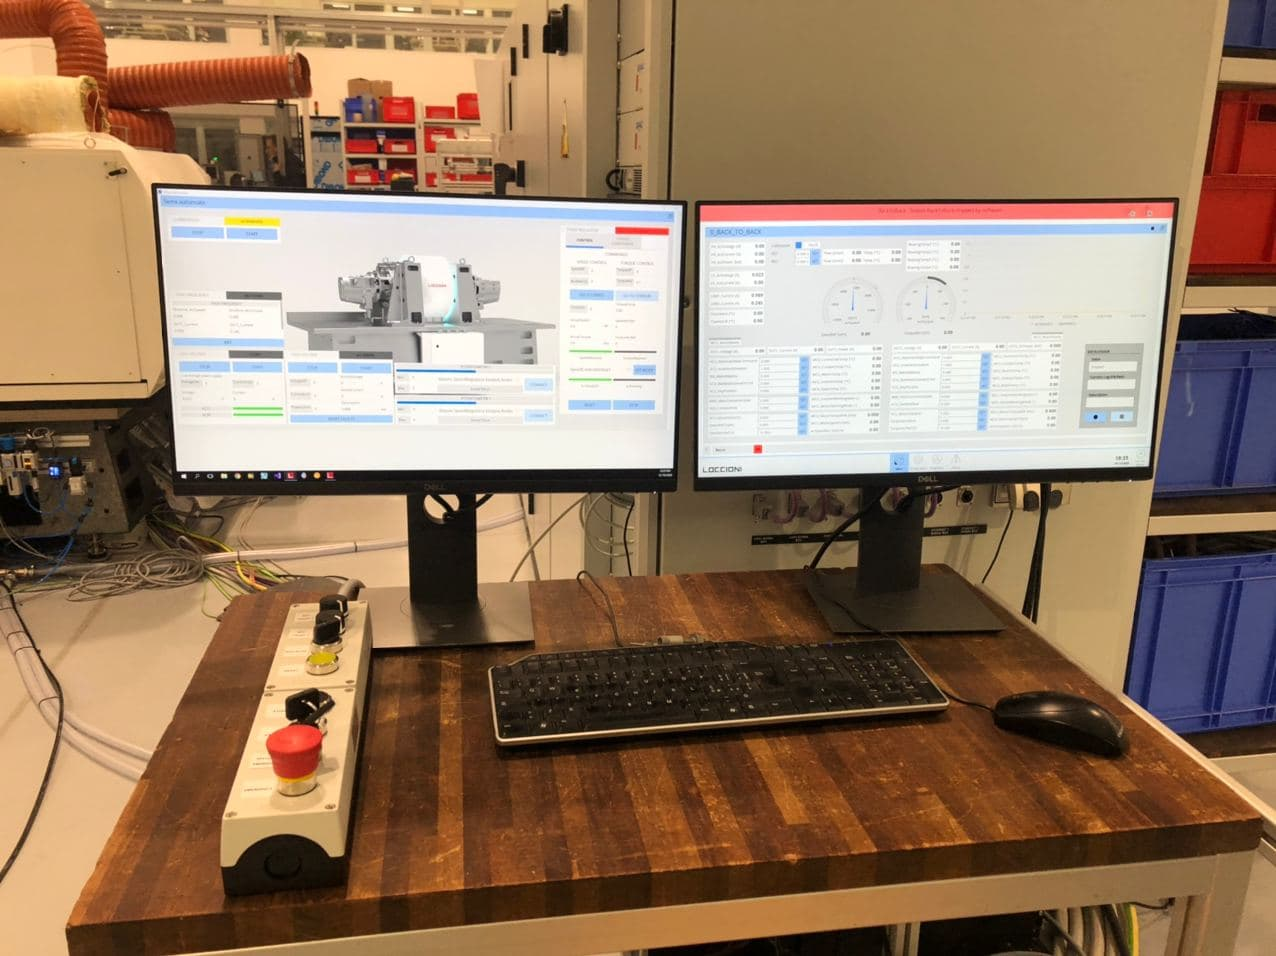
\includegraphics[width=0.5\textwidth]{Postazione}
\caption{Postazione banchi attuale}
\end{figure}

Queste problematiche verrebbero risolte attraverso il Dial, in quanto presenta una “corsa” illimitata, un feedback atpico personalizzabile in base alle operazioni che si svolgono, una precisione laser a 3600 punti e la possibilitá di interagire direttamente con lo schermo, appoggiando il Dial su di esso, permettendo quindi una serie di combinazioni di utilizzo estremamente vasta.

\section{Considerazioni}
Terminata la fase di analisi, in concordato con i nostri tutor aziendali, abbiamo scelto tra le varie tecnologie disponibili, un applicazione UWP in quanto ci ha permesso di utilizzare le librerie native del dispositivo Dial e contemporaneamente un supporto costante da parte di Microsoft.\\

A sostegno di ciò, durante la fase di sviluppo, una difficoltà riscontrata è stata l'assenza di una console di debug web all'interno della WebView impedendoci di verificare il corretto funzionamento della comunicazione bidirezionale, ma grazie al continuo rilascio e aggiornamento da parte della community Micosoft di componenti UWP abbiamo a disposizione una nuova versione della webView rilasciata in versione beta a fine Novembre che consente, oltre a varie migliorie, anche l'utilizzo di una console di debug per lo sviluppo.\\

Un' ulteriore difficoltà riscontrata durante la fase di sviluppo nasce dal fatto che la documentazione presente non trattava in maniera specifica l'utilizzo del dispositivo Dial nel nostro contesto.
Le librerie fornite prevedono la sola integrazione con applicazioni native rendendoci, fino a prova contraria, i primi ad integrarlo in un contesto web, mantenendo però tutte le funzionalità native utilizzabili.\\

Un problema riscontrato nell'utilizzo di un'applicazione UWP con una pagina web caricata al suo interno era quello di riuscire ad implementare una comunicazione bidirezionale efficiente tra due linguaggi di programmazione differenti.

Per risolvere questa problematica ci siamo trovati davanti a due possibilitá:

\begin{enumerate}
\item Utilizzare la funzionalitá della WebView chiamata ScriptNotify che permette la notifica all'applicazione UWP dell'avvenuta emissione di un determinato evento nella pagina Web.
\item Utilizzare il decoratore AllowForWeb su una classe, affinché un'istanza di essa, possa essere iniettata nella pagina Web.
\end{enumerate}

Dopo aver letto la documentazione e effettuato vari test, la scelta è ricaduta sul decoratore AllowForWeb, in quanto lo ScriptNotify permetteva di mettersi in ascolto di solamente un determinato evento e permetteva il ritorno di una sola stringa come parametro.
Inoltre, leggendo su varie Community come StackOverflow, questa pratica viene sconsigliata poiché non sicura, in quanto va necessariamente abilitato lato UWP l'URI di ogni singola pagina da controllare e limitandone l'utilizzo in termini di prestazioni.\\ 

In contrapposizione, utilizzare AllowForWeb su di una classe e iniettare un'istanza nella pagina, ci ha permesse un maggior controllo della comunicazione tra Web e UWP grazie all'utilizzo dei metodi messi a disposizione dall'oggetto, permettendoci di scambiare maggiori informazioni e parametri tipati e non solamente stringhe.\\

\section{Sviluppi Futuri}

I possibili sviluppi sono molteplici e un’idea iniziale è quella di inserire un nuovo widget all’interno della dashboard Loccioni in grado di raffigurare attraverso un’immagine, una parte del motore o un componente da controllare, in modo tale da avere un’interfaccia più intuitiva per la selezione, e successivamente, una volta acquisito il widget stesso, avere la possibilità di visualizzare i dettagli e le funzionalità del componente attraverso il menù del Dial.\\

Uno sviluppo futuro sicuramente necessario è l’aggiunta di un controllo sui dati in input lato web, che momentaneamente non è presente nei nostri widget, ma è fatta solamente lato backend.\\

Per aumentare l'utilizzabilità dell’interfaccia utente è sicuramente necessaria una modifica degli widget da noi creati, per renderli più facilmente selezionabili dal Dial e per migliorare anche l’aspetto visivo.

Il servizio implementato presenta una violazione del principio di singola responsabilità in quanto oltre a gestire la comunicazione bidirezionale con l'applicazione UWP, si occupa anche di tenere traccia di quale Widget presente nella Dashboard é stato acquisito dal Dial in fase di RunMode, escludendo l'ascolto dell'invoke sui suoi canali.
Pertanto, abbiamo pianificato di spostare questa seconda responsabilitá, creando un nuovo servizio dedicato a questo compito.

Qualora il progetto arrivi al punto di essere utilizzato e rilasciato in ambienti industriali, per migliorare la manipolazione di dati modificabili nelle dashboard attuali sará necessario apportare alcune modifiche alla dashboard, per consentire un utilizzo attraverso il touchscreen di un qualsiasi dispositivo, in modo tale da rendere veramente fluido l’utilizzo di tutto l’ambiente e poter così eliminare il mouse dalle operazioni svolte più frequentemente o che richiedono una maggior precisione nella variazione dei dati.\\



\section{Evoluzioni dello State of Art}


Al momento dello sviluppo, la necessitá di dover passare per un applicazione UWP rappresenta sicuramente una limitazione che andrá tolta qualora il progetto verrá rilasciato in ambito industriale.\\

A favore di questa considerazione, nel mese passato, la Google stessa ha rilasciato in fase di Preview una libreria Web chiamata Trial for WebHID, la quale permetterá di far comunicare direttamente con la pagina Web i dispositivi che utilizzano il protocollo HID, come il Dial, permettendo agli sviluppatori futuri di non dover necessariamente passare attraverso una WebView o una applicazione nativa per quel dispositivo.\\

-HID nel web utilizzo
-Cloud game -> utilizzo potenza di calcolo esterna all'hardware
-Microsoft spinge sul web con webview2
-portabilità








\appendix
%\input{schema_elettrico}
%\input{Appendix1}
%\input{Appendix2}

\printbibliography

\printindex

\chapter*{Ringraziamenti}



\end{document}